%%%%%%%%%%%%%%%%%%%%%%%%%%%%% ANEXO %%%%%%%%%%%%%%%%%%%%%%%%%%%%%

%\section*{\centering{A – ANEXOS Y APÉNDICES }} % Añadir código
%\addcontentsline{toc}{section}{A - ANEXOS Y APÉNDICES}

% Los anexos y apéndices son materiales adicionales, utilizados para complementar el texto, añadidos al final del trabajo, con la finalidad de aclaración o de comprobación. Son elaborados por el autor y pretenden complementar una argumentación y sirven de fundamentación teórica, comprobación e ilustración (por ejemplo, mapas, leyes, códigos)

%\chapter*{Apendice A - }
%\label{ch:Apendice}

%\section*{\huge Apéndice A} 
%\section*{Fuentes de información para la descarga de MDT}
%\addcontentsline{toc}{chapter}{Apéndice A: Fuentes de información para descarga de MDT}

%\begin{itemize}
%	\item \item \url{https://www.cursosteledeteccion.com/fuentes-gratuitas-para-descargar-dem-modelo-de-elevacion-digital/}
%	\item \url{http://www.gisandbeers.com/descarga-de-dem-mundiales-mde/}
%	\item \url{https://gisgeography.com/free-global-dem-data-sources/}
%	\item \url{http://www.gpsvisualizer.com/elevation}
%	\item \url{https://mappinggis.com/2017/12/programas-gratuitos-para-trabajar-con-imagenes-de-satelite/}
%\end{itemize}

\newpage

\section*{\huge Apéndice A} 
\section*{Evolución de la Web}
\label{ch:ApendiceA}
\addcontentsline{toc}{chapter}{Apéndice A: Evolución de la Web}

\subsection{Tipos de Web} % Evolución de la Web

\section{Linked Data}
3.1 
285/5000

% http://www.fgcsic.es/lychnos/es_es/articulos/construyendo_una_web_semantica
El potencial de la web de datos, al igual que pasó con la web de documentos, reside en la participación a gran escala de numerosas personas y organizaciones en la publicación sistemática de datos en la Web, siguiendo las buenas prácticas de Linked Data. Es esta participación masiva, con un esfuerzo relativamente bajo, la que está detrás del éxito de la Web actual. La publicación de datos es solo una parte de lo que constituye la web de datos. La otra parte la forman las aplicaciones informáticas que nos proveen de los servicios para acceder, consultar, buscar y combinar los datos. 


\begin{figure}
	\centering
	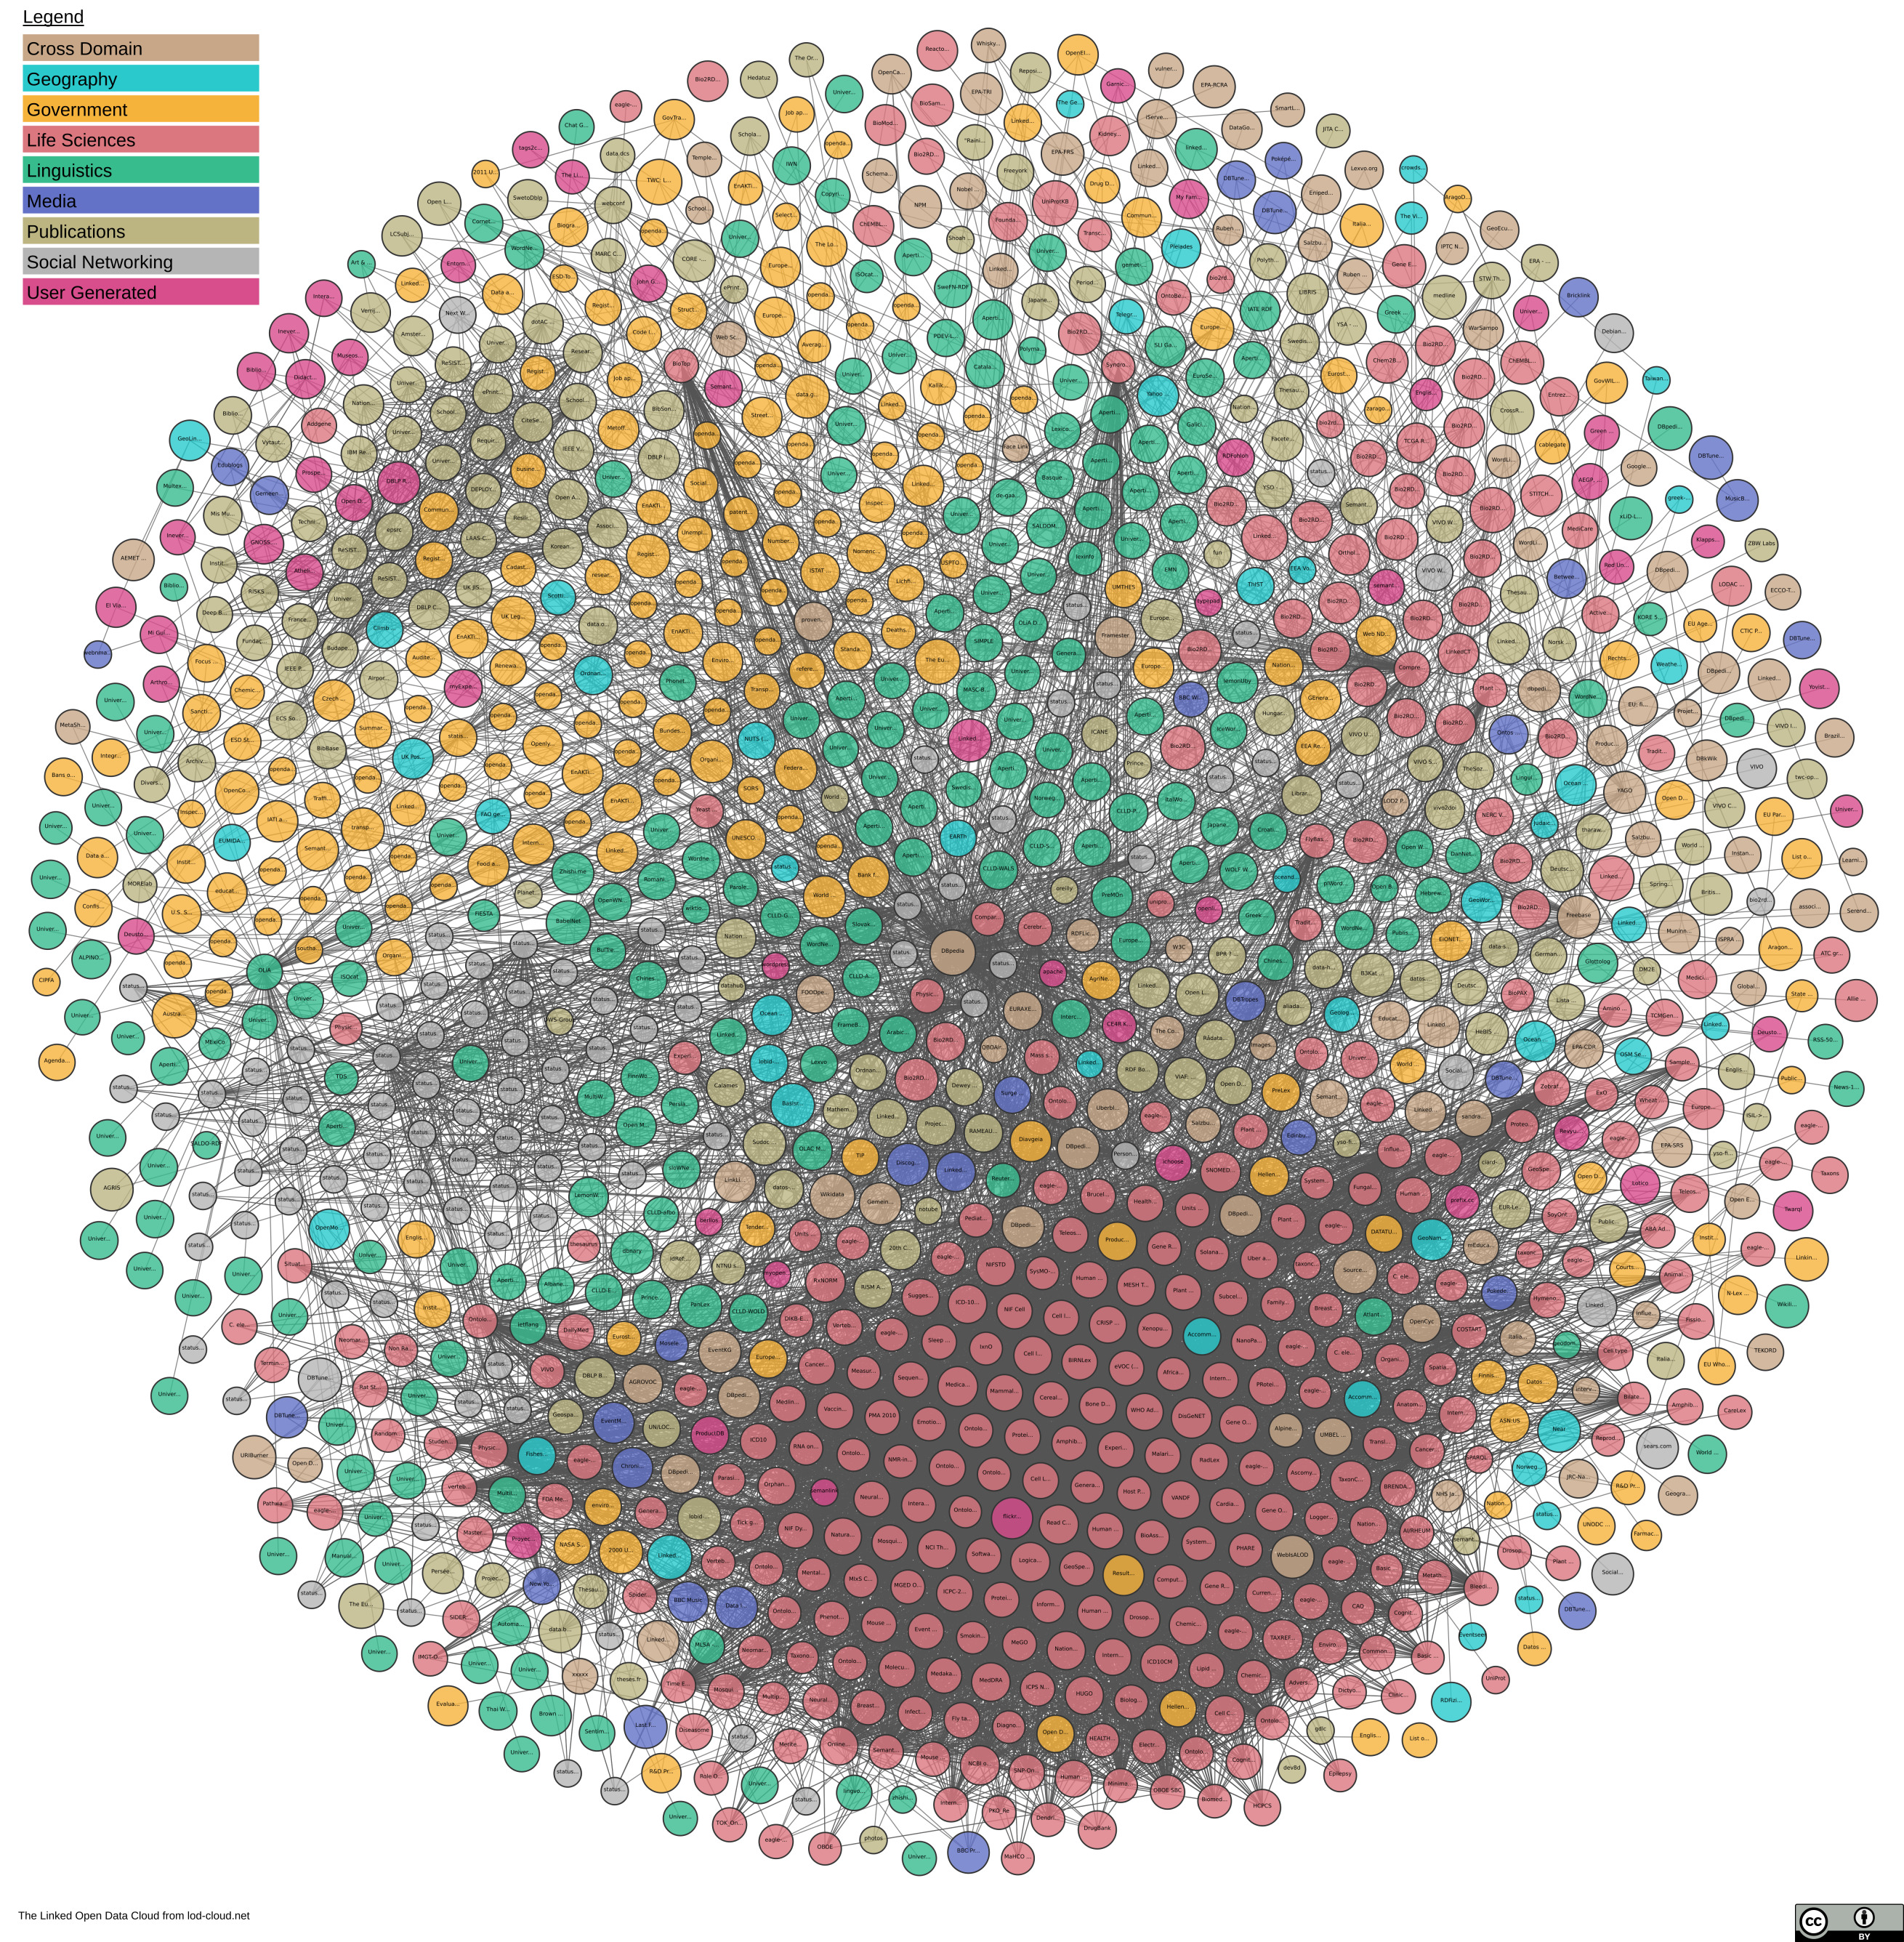
\includegraphics[width=0.7\linewidth]{imagenes/capitulo3/lod-cloud-sm}
	\caption{}
	\label{fig:lod-cloud-sm}
\end{figure}

%tesis
Para lograr publicar información  en la Web de datos, es necesario, primero disponer de un repositorio donde almacenarlos y consultarlos; y segundo, la información  debe estar en el formato adecuado (RDF). Sin embargo, para el primer requerimiento, no existe un repositorio del Ecuador donde externamente se puede enlazar datos, sino actualmente cada institución (empresa, persona) publica su propia información  sin relacionarla (aun teniendo información  que puede ser complementaria), dicha información  tampoco puede ser tratada mediante consultas semánticas, por ejemplo consultas semánticas geoespaciales (funciones GEOSPARQL). Para el segundo requerimiento, el inconveniente es la falta de herramientas de fácil uso (preferiblemente con interfaz gráfica) para la generación de RDF y que sea compatible con el estándar GEOSPARQL . 

%tesis
Pero incluso, si se llega a obtener de esta manera la información , la misma no estaría relacionada, y peor aún, visible por otros grandes repositorios de datos como la DBpedia

\section{title}
Fuentes de datos espaciales semánticas interesantes
Hay muchas fuentes de datos que se ajustan a los datos vinculados, consulte la Fig. 3.1. Elegiré y describiré algunos de ellos, que son relevantes para esta tesis, los que contienen algún tipo de información espacial. Se usan para mi prototipo en el Capítulo 5.





